\documentclass[13pt,a4paper]{article}
\usepackage[spanish,es-nodecimaldot]{babel}	% Utilizar español
\usepackage[utf8]{inputenc}					% Caracteres UTF-8
\usepackage{graphicx}						% Imagenes
\usepackage[hidelinks]{hyperref}			% Poner enlaces sin marcarlos en rojo
\usepackage{fancyhdr}						% Modificar encabezados y pies de pagina
\usepackage{float}							% Insertar figuras
\usepackage[textwidth=390pt]{geometry}		% Anchura de la pagina
\usepackage[nottoc]{tocbibind}				% Referencias (no incluir num pagina indice en Indice)
\usepackage{enumitem}						% Permitir enumerate con distintos simbolos
\usepackage[T1]{fontenc}					% Usar textsc en sections
\usepackage{amsmath}						% Símbolos matemáticos
\usepackage[ruled,vlined]{algorithm2e}      % Pseudocódigo
\usepackage{xcolor}
\usepackage{listings}
% Para que acepten tíldes los listing
\lstset{     
     literate=%
         {á}{{\'a}}1
         {é}{{\'e}}1
         {í}{{\'i}}1
         {ó}{{\'o}}1
         {ú}{{\'u}}1
         {Á}{{\'A}}1
         {É}{{\'E}}1
         {Í}{{\'I}}1
         {Ó}{{\'O}}1 
         {Ú}{{\'U}}1
         {ñ}{{\~n}}1 
         {Ñ}{{\~N}}1 
         {¿}{{?``}}1 
         {¡}{{!``}}1
}
\usepackage{dsfont}

% ==============================================================================

\usepackage{caption, subcaption}
\usepackage[section]{placeins}
\makeatletter
\def\fps@figure{H}
\makeatother

\usepackage{booktabs}
\usepackage{longtable}
\usepackage{array}
\usepackage{multirow}
\usepackage{wrapfig}
\usepackage{colortbl}
\usepackage{pdflscape}
\usepackage{tabu}
\usepackage{threeparttable}
\usepackage{threeparttablex}
\usepackage[normalem]{ulem}
\usepackage{makecell}
\usepackage{xcolor}
\usepackage[bottom]{footmisc}

\makeatletter
\newcommand*{\centerfloat}{%
  \parindent \z@
  \leftskip \z@ \@plus 1fil \@minus \textwidth
  \rightskip\leftskip
  \parfillskip \z@skip}
\makeatother

% ==============================================================================
% ==============================================================================

% Comando para poner el nombre de la asignatura
\newcommand{\asignatura}{Visión por Computador}
\newcommand{\autor}{Ignacio Vellido Expósito}
\newcommand{\email}{ignaciove@correo.ugr.es}
\newcommand{\titulo}{Cuestiones}
\newcommand{\subtitulo}{1}

% Configuración de encabezados y pies de pagina
\pagestyle{fancy}
\lhead{\autor{}}
\rhead{\asignatura{}}
\lfoot{Máster Ciencia de Datos e Ingeniería de Computadores}
\cfoot{}
\rfoot{\thepage}
\renewcommand{\headrulewidth}{0.4pt}		% Linea cabeza de pagina
\renewcommand{\footrulewidth}{0.4pt}		% Linea pie de pagina

% ==============================================================================
% ==============================================================================

\begin{document}
    \pagenumbering{gobble}
    % ==============================================================================
% Pagina de titulo
\begin{titlepage}
    \begin{minipage}{\textwidth}
        \centering

        
\includegraphics[scale=0.5]{img/ugr.png}\\

        \textsc{\Large \asignatura{}\\[0.2cm]}
        \textsc{MÁSTER CIENCIA DE DATOS E INGENIERÍA DE COMPUTADORES}\\[1cm]

        \noindent\rule[-1ex]{\textwidth}{1pt}\\[1.5ex]
        \textsc{{\Huge \titulo\\[0.5ex]}}
        \textsc{{\Large \subtitulo\\}}
        \noindent\rule[-1ex]{\textwidth}{2pt}\\[2.5ex]

        \end{minipage}

        \vspace{0.3cm}

        \begin{minipage}{\textwidth}

        \centering

        \textbf{Autor}\\ {\autor{} \\ ignaciove@correo.ugr.es}\\[1.5ex]
        \vspace{0.4cm}

        
\includegraphics[scale=0.3]{img/etsiit.jpeg}
        
\includegraphics[scale=0.6]{img/master.png}

        \vspace{0.7cm}
        \textsc{Escuela Técnica Superior de Ingenierías Informática y de Telecomunicación}\\
        \vspace{1cm}
        \textsc{Curso 2020-2021}
    \end{minipage}
\end{titlepage}
% ==============================================================================
    
    % \pagenumbering{arabic}
    % \tableofcontents
    % \thispagestyle{empty}				% No usar estilo en la pagina de indice

    \newpage

    % ==============================================================================

    % \section{Resultados globales}

Orden usado en las técnicas:
Under/Oversampling > NoiseFiltering > Instance Selection

\begin{figure}[ht]
    \centerfloat
    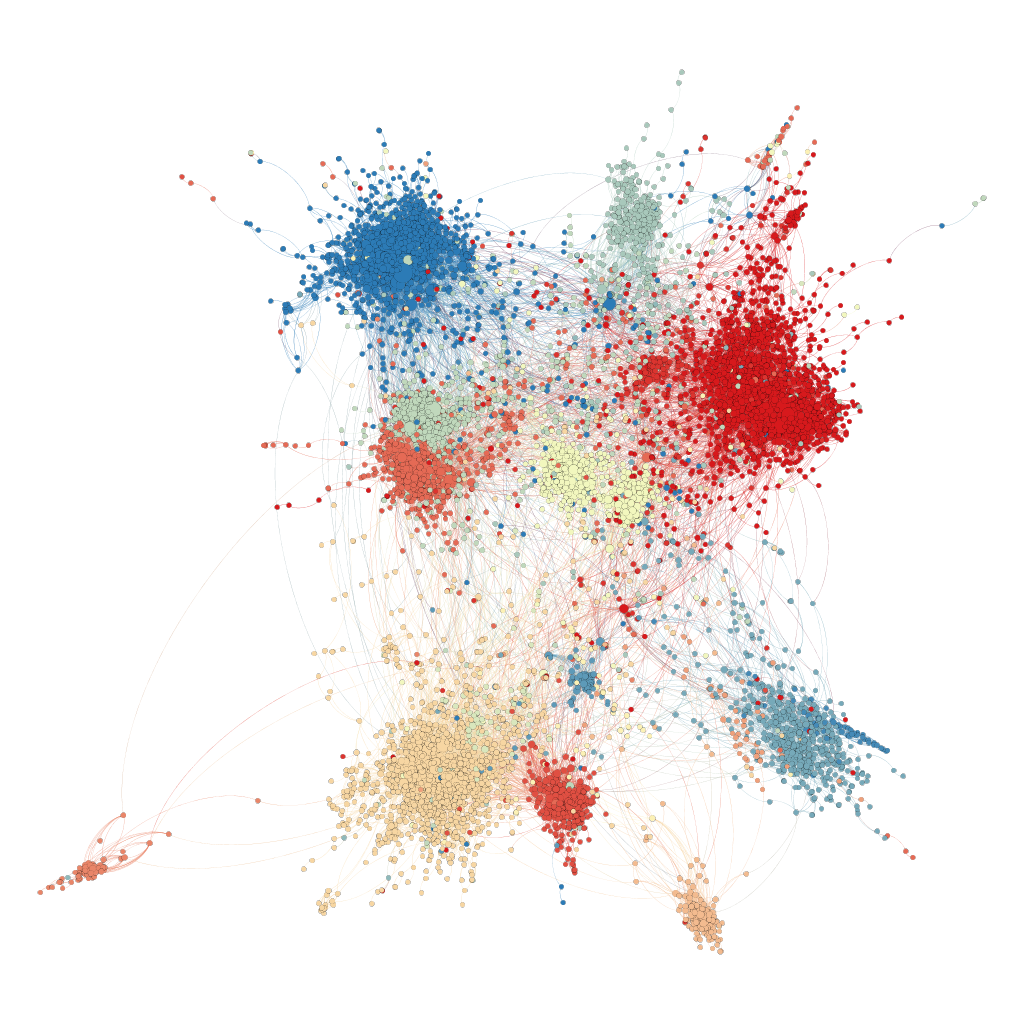
\includegraphics[width=1.097\textwidth]{img/resultados/grado-targets.png}
    \caption{Topología de la red. El color indica el país de cada usuario.}
\end{figure}

\begin{figure}[t]
    \centering
    \resizebox{0.78\columnwidth}{!}{%
    \begin{tabular}{| l | r |} 
        \hline
        \textbf{Medida} & \textbf{Valor} \\
        \Xhline{2\arrayrulewidth}
        Número de nodos \textbf{N} & 7,624 \\
        \hline
        Número de enlaces \textbf{L}	& 27,806 \\
        \hline
        Número máximo de enlaces \textbf{$L_{max}$} & 58117752 \\
        \hline
        Densidad del grafo \textbf{$L/L_{max}$} & 0.001 \\
        \Xhline{2\arrayrulewidth}
        Grado medio \textbf{<k>} & 7.294 \\
        \hline
        Diámetro \textbf{$d_{max}$} & 15 \\
        \hline
        Distancia media \textbf{d} & 5.232237269 \\
        \hline
        Coeficiente medio de clustering \textbf{<C>} & 0.285 \\
        \Xhline{2\arrayrulewidth}
        Número de componentes conexas & 1 \\
        \hline
        Número de nodos componente gigante (y \%) & 7,624 (100) \\
        \hline
        Número de aristas componente gigante (y \%) & 27,806 (100) \\
        \hline
    \end{tabular}
    }
    \caption{Medidas globales de la red.}
\end{figure} \newpage

\begin{enumerate}  
  \item \textbf{¿Qué es una imagen?}
  
  La representación de una escena tridimensional en un espacio bidimensional.

  La mayor parte de las imágenes que percibimos provienen de una fuente de luz reflejada sobre objetos en un espacio 3D sobre una superficie fotosensible, aunque también existen imágenes generadas por emisión y absorción.
  \item \textbf{¿En qué consiste el proceso de digitalización?}

  El objetivo de la digitalización es la discretización de los valores continuos de una imagen. Para ello se elige el rango de muestreo (número de puntos que codifican la imagen); el formato de cuantificación (el rango de valores usado para codificar); y el patrón de teselación (tamaño y forma) en el que dividir la imagen.
  \item \textbf{¿Qué diferencias hay entre cuantificación y muestreo?}

  Se tratan de procesos diferentes, que no se oponen sino que se complementan. El muestreo determina la cantidad de muestras (o puntos) que codifican la imagen, mientras que la cuantificación indica los posibles valores que pueden tomar estas muestras.

  Por ejemplo, para una imagen digital usaríamos el muestreo para determinar la resolución (número de píxeles) y con la cuantificación la codificación del color o nivel de gris (transformación de los valores continuos de la señal en niveles discretos).
  \item \textbf{Si en la imagen el objeto más pequeño mide 10 pixeles, ¿cual sería el tamaño de muestreo que necesitamos para representar esa estructura?}

  El intervalo de muestreo para preservar perfectamente ese objeto debe ser como máximo de $\frac{10}{2} = 5$ pixeles.
  \item \textbf{Si tenemos 20 tonos de niveles de gris para el proceso de cuantificación ¿cuantos bits necesitamos para representar cada pixel?}

  $2^{5} = 32 > \textbf{20} > 16 = 2^{4}$ 
  
  \textbf{5 bits}, y nos sobrarían 12 posibles niveles de gris adicionales que podríamos representar con la misma cantidad. 
  \item \textbf{Comentar si son verdaderas o falsas la siguientes afirmaciones:}
    \begin{enumerate}
      \item \textbf{En el modelo de cámara “pinhole” debemos tener una apertura grande.}

      La apertura en sí debe tener un tamaño pequeño, pero puede ser más o menos grande en base a la distancia del objeto que estemos interesados en observar.
      Si la apertura es demasiado grande más de un rayo del mismo punto 3D real se reflejará sobre distintos puntos del plano de proyección, emborronando la imagen.
      Por otro lado si es demasiado pequeña se genera saturación por la excesiva exposición de rayos en el mismo punto del plano de proyección.      
      \item \textbf{La distancia focal es la distancia que existe entre el agujero, en el modelo de cámara pinhole, y el plano de proyección.}

      Exacto, concretamente la distancia entre el agujero y el punto central del plano de proyección.
      \item \textbf{Un punto P en el mundo real en un modelo de cámara ideal, se proyecta en un único punto en el plano de imagen.}

      Verdadero en un modelo de cámara ideal, ya que la proyección en un único punto de multiples rayos reflejados generaría emborronamiento.
      \item \textbf{Un punto P en el plano de imagen se proyecta en un único punto en el mundo real.}

      Falso, un punto P se proyecta como una línea pasando por punto focal, resultando en múltiples posibles puntos reales a diferentes distancias de la cámara.
    \end{enumerate}
  \item \textbf{¿Cuál es el sistema de representación de color que representa el color como lo hace el humano?}

  La retina humana contiene unos receptores llamados \textit{conos} que responden a las diferentes longitudes de onda de la luz. Existen tres tipos activados por diferentes longitudes, y asociados a cada uno de los colores primarios. Las visualización del resto de colores se forma por la combinación en diferentes intensidades de varios colores primarios.

  \begin{figure}[h]
    \centerfloat
    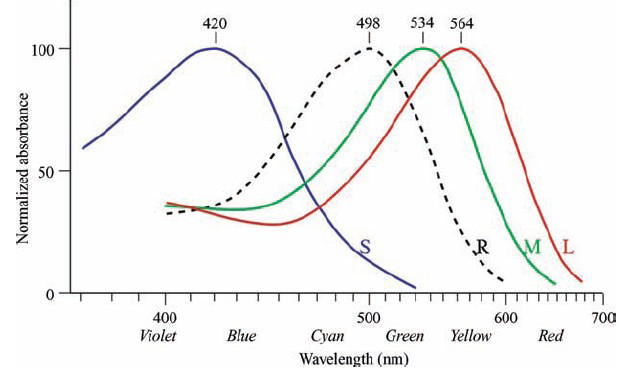
\includegraphics[width=0.75\textwidth]{img/conos.png}
    % \caption{Relación intermediación-vector propio en escala logarítmica.}
  \end{figure}
\end{enumerate}

    % ==============================================================================

    \setlength{\parskip}{1em}
    \newpage
    % \nocite{*}
    % \bibliography{bibliografia}
  	% \bibliographystyle{plain}
\end{document}